
\subsection{利用者の管理とアクセス制御システムの整備}
独立した運用を行うためには利用者の管理とアクセス制御システムの整備が必要である.
既存の滞在ウォッチは単独コミュニティでのみの運用を前提としており開発者と管理者が同一であった.
また利用者の権限に関する情報とそれに基づいたWebページログインの仕組みが存在せず,在室情報はプライバシに関わるものだが誰でも閲覧可能な状態であった.
しかし複数コミュニティ間で運用を行う場合,コミュニティの数が増えるに連れてシステム開発者の利用者管理の負担が大きくなり運用するのは難しくなる.
これを解決するには各コミュニティごとに管理者を作り,各コミュニティで独立した運用を行う必要がある.
各コミュニティごとに管理者が存在すればコミュニティの利用者の管理を全て行う必要がないため開発者の負担が軽減される.

そこでGoogleアカウントを用いた利用者の認証機能を実装した.
Googleアカウントを用いた認証のみでは,アカウント自体に滞在ウォッチに関する権限情報がないため利用者の識別はできない.
そのため利用者の権限情報とアカウントを滞在ウォッチデータベースの利用者情報と紐づけている.
これによりアカウントでログインしている利用者が管理者であるかの識別が可能である.

また管理者が利用者の登録を行える仕組みを作成した.
利用者はシステム上にログインし,管理者にログインを行ったアカウントを報告する.
管理者が図2に示すWebページの利用者登録画面からそれを登録すると滞在ウォッチデータベースに利用者情報とGoogleアカウントが登録される.
利用者がログインした上でWebページを閲覧する際にWebページ側から利用者のアカウント情報を滞在ウォッチAPIサーバに送る.
その後データベースにそのアカウントが登録されているかを確認する.
登録されている場合はWebページに対してその利用者の在室情報の閲覧の許可を与える.
仮に外部のものがGoogleアカウントを使ってログインしたとしてもデータベースにそのアカウントが登録されていないため在室情報の閲覧は不可能である.
これにより適切な範囲での在室情報を扱うことが可能である.


\begin{figure}[tbh]
  \centering
  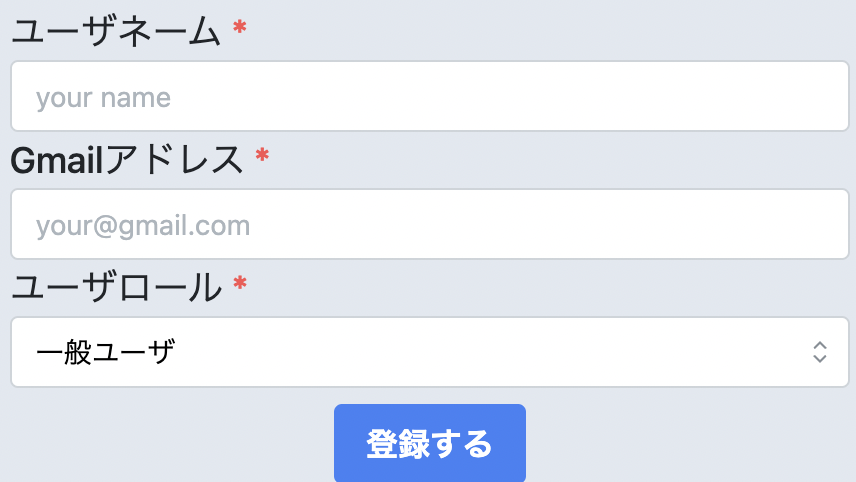
\includegraphics[width=6cm]{image/register.png}
  \caption{利用者登録画面}
  \label{multipleBPM}
\end{figure}